\documentclass[12pt,a4paper,oneside,fleqn,leqno]{article}
\usepackage[utf8]{inputenc}
\usepackage[T1]{fontenc}
\usepackage{geometry}
\usepackage{graphicx}
\usepackage{amssymb}
\usepackage{amsmath}
\usepackage{wrapfig}
\usepackage{float}
\usepackage{caption}
\usepackage{subcaption}
\usepackage{multirow}
\usepackage{listings}
\usepackage{epstopdf}
%\usepackage[center]{caption}
\geometry{a4paper}
\usepackage[russian]{babel}

\setlength{\topmargin}{-1.0in}
\setlength{\textheight}{10.5in}
\setlength{\oddsidemargin}{-.125in}
\setlength{\textwidth}{6.5in}

\begin{document}
	\begin{titlepage}
		\begin{center}
			\large Московский государственный университет им.\,М.\,В.\,Ломоносова\\
			Факультет вычислительной математики и кибернетики \\
			Кафедра математических методов прогнозирования \\[4.5cm] 
			\Huge Задание \No\,1.\\Вероятностные модели посещаемости курса\\[5.5cm]
		\end{center}
		\normalsize
		\begin{flushright}
			\emph{Автор:} Арбузова Дарья\\
			\emph{Группа:} 417\\
		\end{flushright}
		\vfill
		\begin{center}
			Москва, 2014
		\end{center}
	\end{titlepage}
	\tableofcontents
	\newpage
	\section{Постановка задачи}
		Рассмотрим модель посещаемости студентами одного курса лекции. Пусть аудитория данного курса состоит из студентов профильной кафедры, а также студентов других кафедр. Обозначим\\
		\begin{minipage}{0.7\textwidth}
		\vspace{10pt}
			\begin{itemize}
				\item
				$a$ --- количество студентов, распределившихся на профильную кафедру;
				\item
				$b$ --- количество студентов других кафедр на курсе;
				\item
				$c$ --- количество студентов на данной лекции;
				\item
				$d$ --- общее количество записавшихся на данной лекции;
				\item
				$p_1$ --- вероятность посещения лекции студентом профильной кафедры;
				\item
				$p_2$ --- вероятность посещения лекции студентом любой из остальных кафедр;
				\item
				$p_3$ --- вероятность, с которой студент записывает своего товарища.
			\end{itemize}
		\end{minipage}
		\begin{minipage}{0.3\textwidth}
			\begin{figure}[H]
				\captionsetup{justification=centering}
				\includegraphics[width=1.0\textwidth]{gm.png}
				\caption{Графическая модель}
				\label{fig:gm}
			\end{figure}
		\end{minipage}

	\begin{minipage}{0.5\textwidth}
		\vspace{10pt}
			В модели 1:
			\begin{itemize}
				\item
				$a \sim R[a_{min}; a_{max}]$
				\item
				$b \sim R[b_{min}; b_{max}]$
				\item
				$c|a,b \sim B(a, p_1) + B(b, p_2)$
				\item
				$d|c \sim c + B(c, p_3)$
			\end{itemize}
		\end{minipage}
		\begin{minipage}{0.5\textwidth}
			В модели 2:
			\begin{itemize}
				\item
				$a \sim R[a_{min}; a_{max}]$
				\item
				$b \sim R[b_{min}; b_{max}]$
				\item
				$c|a,b \sim Poiss(ap_1 + bp_2)$
				\item
				$d|c \sim c + B(c, p_3)$
			\end{itemize}
		\end{minipage}
		\vspace{10pt}\par
		Значения параметров: $a_{min} = 15, a_{max} = 30, b_{min} = 250, b_{max} = 350, p_1 = 0.5, p_2 = 0.05, p_3 = 0.5.$\par
		В данном задании необходимо исследовать поведение моделей при различных параметрах, а также оценить плотность некоторых распределений с приходом новой информации.
	\section{Вывод формул для расчёта распределений}
			Проведём вывод необходимых распределений для рассматриваемых моделей, пользуясь фактами из теории вероятностей:
			\begin{enumerate}
				\item $a \sim R[a_{min}; a_{max}]$
				$$p(a) = \frac{1}{a_{max} - a_{min} + 1}$$
				$$\mathbb{E}[a] = \frac{a_{min} + a_{max}}{2}$$
				$$\mathbb{D}[a] = \frac{(a_{max} - a_{min} + 1)^2 - 1}{12}$$
				%\noindent\makebox[\linewidth]{\rule{\textwidth}{0.4pt}}
				\item $b \sim R[b_{min}; b_{max}]$ аналогично:\\
				$$p(b) = \frac{1}{b_{max} - b_{min} + 1}$$
				$$\mathbb{E}[b] = \frac{b_{min} + b_{max}}{2}$$
				$$\mathbb{D}[b] = \frac{(b_{max} - b_{min} + 1)^2 - 1}{12}$$
				%\noindent\makebox[\linewidth]{\rule{\textwidth}{0.4pt}}
				\item $b|a$
				$$ p(b|a) = \frac{p(a, b)}{p(a)} = \frac{\sum\limits_{c = 0}^{a + b} \sum\limits_{d = c}^{2c} p(a, b, c, d)}{p(a)} = p(b) \cdot \sum\limits_{c = 0}^{a + b} p(c|a, b) \cdot \sum\limits_{d = c}^{2c} p(d|c) = p(b)$$
				Величины $a$ и $b$ независимы в рамках рассматриваемых моделей.
				%\noindent\makebox[\linewidth]{\rule{\textwidth}{0.4pt}}
				\item 
				\begin{enumerate}
					\item Модель 1: $c|a,b \sim B(a, p_1) + B(b, p_2)$\\
					Пусть $c = x + y,$ где $x \sim B(a, p_1), y \sim B(b, p_2),$ тогда
					$$p(c|a,b) = \sum_{k = 0}^c p(x = k; a, p_1) \cdot p(y = c - k; b, p_2) = $$ $$
				=\sum_{k = 0}^c C_a^k p_1^k (1 - p_1)^{a - k} \cdot C_b^{c - k} p_2^{c - k} (1 - p_2)^{b + k - c}$$
					\item Модель 2: $c|a,b \sim Poiss(ap_1 + bp_2)$
					$$p(c|a,b) = e^{\lambda}\frac{\lambda^c}{c!},$$ где $\lambda = ap_1 + bp_2.$
				\end{enumerate}
				\item $d|c \sim c + B(c, p_3)$
				$$ p(d|c) = C_{c}^{d - c}p_3^{d - c}(1 - p_3)^{2c - d}$$
				%\noindent\makebox[\linewidth]{\rule{\textwidth}{0.4pt}}
				\item $c|a$
				$$p(c|a) = \frac{p(a, c)}{p(a)} = \frac{\sum\limits_{b = b_{min}}^{b_{max}} \sum\limits_{d = 0}^{2(a + b)}p(a, b, c, d) }{p(a)} = $$ $$ = p(b) \cdot \sum\limits_{b = b_{min}}^{b_{max}} p(c|a, b) \cdot \sum\limits_{d = 0}^{2(a + b)}p(d|c) = p(b) \cdot \sum\limits_{b = b_{min}}^{b_{max}} p(c|a, b)$$
				\item $c|b$ аналогично:
				$$p(c|b) = p(a) \cdot \sum\limits_{a = a_{min}}^{a_{max}} p(c|a, b)$$
				%\noindent\makebox[\linewidth]{\rule{\textwidth}{0.4pt}}
				\item $c$
						$$p(c) = \sum\limits_{a = a_{min}}^{a_{max}} \sum\limits_{b = b_{min}}^{b_{max}} \sum\limits_{d = 0}^{2(a + b)} p(a, b, c, d) =$$ 
						$$ = p(a) \cdot p(b) \cdot \sum\limits_{a = a_{min}}^{a_{max}} \sum\limits_{b = b_{min}}^{b_{max}} p(c|a,b) \cdot \sum\limits_{d = 0}^{2(a + b)} p(d|c) = p(a)\cdot p(b) \cdot  \sum\limits_{a = a_{min}}^{a_{max}} \sum\limits_{b = b_{min}}^{b_{max}} p(c|a,b)$$
				%\noindent\makebox[\linewidth]{\rule{\textwidth}{0.4pt}}
				\item $d$
				$$ p(d) = \sum\limits_{c = 0}^{a_{max} + b_{max}}p(d|c)p(c)$$
				%\noindent\makebox[\linewidth]{\rule{\textwidth}{0.4pt}}
			\end{enumerate}
		\section{Априорные распределения}
			Требуется рассчитать математические ожидания и дисперсии априорных распределений $a, b, c$ и $d$.\par
			Пусть для некоторый случайной величины $x$ известно её распределение, тогда
			$$ \mathbb{E}[x] = \sum_{x = x_{min}}^{x_{max}}xp(x)$$
			$$ \mathbb{D}[x] = \sum_{x = x_{min}}^{x_{max}}x^2p(x) - (\mathbb{E}[x])^2$$\par
			В пункте 2 было показано, как получить априорные распределения, имея $p(c|a,b)$ и $p(d|c).$\par
			Результаты приведены в таблице \ref{tab:aprior} (прочерк означает одинаковое поведение в обеих моделях):
			\begin{table}[H]
			\centering
			\begin{tabular}{|c|c|c|c|c|}
				\hline
				\multirow{2}{*}{Величина} & \multicolumn{2}{c|}{Модель 1} & \multicolumn{2}{c|}{Модель 2}\\
				\cline{2-5}
				 & $\mathbb{E}$ & $\mathbb{D}$ & $\mathbb{E}$ & $\mathbb{D}$\\
				\hline
				a & 22.5 & 21.25 & - & -\\
				\hline
				b & 300 & 850 & - & -\\
				\hline
				c & 26.25 & 27.3125 & - & 33.6875\\
				\hline
				d & 39.375 & 68.0156 & - & 82.3594\\
				\hline
				\end{tabular}
			\caption{Априорные распределения}
			\label{tab:aprior}
		\end{table}\par
		Приведём вид исследованных распределений на графиках ниже (см. рис. \ref{fig:bla}):
			\begin{figure}[H]
				\begin{subfigure}[b]{0.5\textwidth}
					\centering
					\includegraphics[width=1.0\textwidth]{p_c.eps}
					\caption{$p(c)$}
					\label{fig:distr_c}
				\end{subfigure}
				\begin{subfigure}[b]{0.5\textwidth}
					\centering
					\includegraphics[width=1.0\textwidth]{p_d.eps}
					\caption{$p(d)$}
					\label{fig:distr_d}
				\end{subfigure}
				\captionsetup{justification=centering}
				\caption{Распределения $p(c)$ и $p(d)$ для моделей 1 и 2}
				\label{fig:bla}
			\end{figure}
		\section{Прогноз величины $b$}
			Требуется пронаблюдать, как происходит уточнение прогноза для величины $b$ с приходом новой информации.\par
			Рассмотрим распределения $b, b|a, b|a,d$. Как было показано выше в пункте 2, $b$ и $b|a$ распределены одинаково, поэтому будем сравнивать только $b$ с $b|a, d$.\par
			На рисунке \ref{fig:distr_b_ad} показано распределение соответствующих величин для моделей 1 и 2, а также указаны их матожидания.
			\begin{figure}[H]
				\captionsetup{justification=centering}
				\includegraphics[width=1.0\textwidth]{p_b_ad.eps}
				\caption{Уточнение прогноза для величины $b$ с приходом новой информации для моделей 1 и 2}
				\label{fig:distr_b_ad}
			\end{figure}
		\section{Влияние параметров $p_1$ и $p_2$}
			Требуется исследовать, каким образом единичный квадрат разбивается на области $\{(p_1, p_2) | \mathbb{D}[c|a] \leqslant \mathbb{D}[c|b] \}$ и $\{(p_1, p_2) | \mathbb{D}[c|a] > \mathbb{D}[c|b] \}$. Результаты для моделей 1 и 2 представлены на рисунках \ref{fig:variance_binary_1} и \ref{fig:variance_binary_2} соответственно.
			\begin{figure}[H]
				\begin{subfigure}[b]{0.5\textwidth}
					\centering
					\includegraphics[width=1.0\textwidth]{variance_binary_1.eps}
					\caption{Модель 1}
					\label{fig:variance_binary_1}
				\end{subfigure}
				\begin{subfigure}[b]{0.5\textwidth}
					\centering
					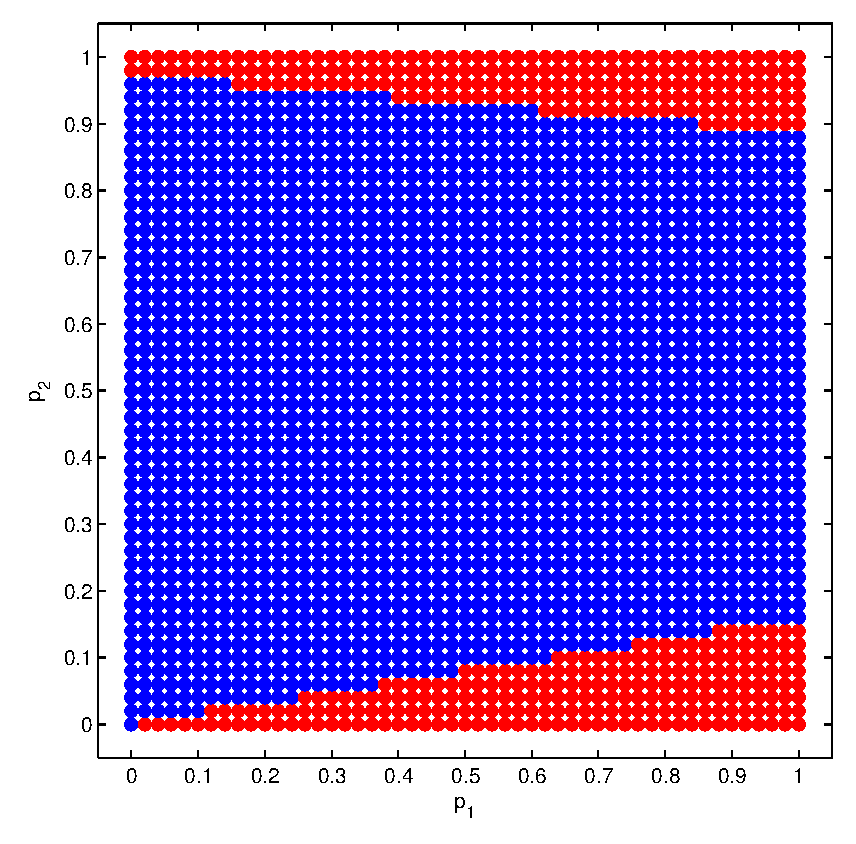
\includegraphics[width=1.0\textwidth]{variance_binary_2.eps}
					\caption{Модель 2}
					\label{fig:variance_binary_2}
				\end{subfigure}
				\captionsetup{justification=centering}
				\caption{Соотношение между $\mathbb{D}[c|a]$ и $\mathbb{D}[c|b]$ в зависимости от $p_1$ и $p_2$ для моделей 1 и 2}
				\label{fig:distr_c_d}
			\end{figure}
\par
			Для большей наглядности рассмотрим трёхмерные графики зависимости $\mathbb{D}[c|a] - \mathbb{D}[c|b]$ от параметров $p_1$ и $p_2$ (рисунки \ref{fig:variance_1} и \ref{fig:variance_2} для моделей 1 и 2 соответственно). Синим обозначена плоскость, соответствующая равенству дисперсий.
			\begin{figure}[H]
				\begin{subfigure}[b]{0.5\textwidth}
					\centering
					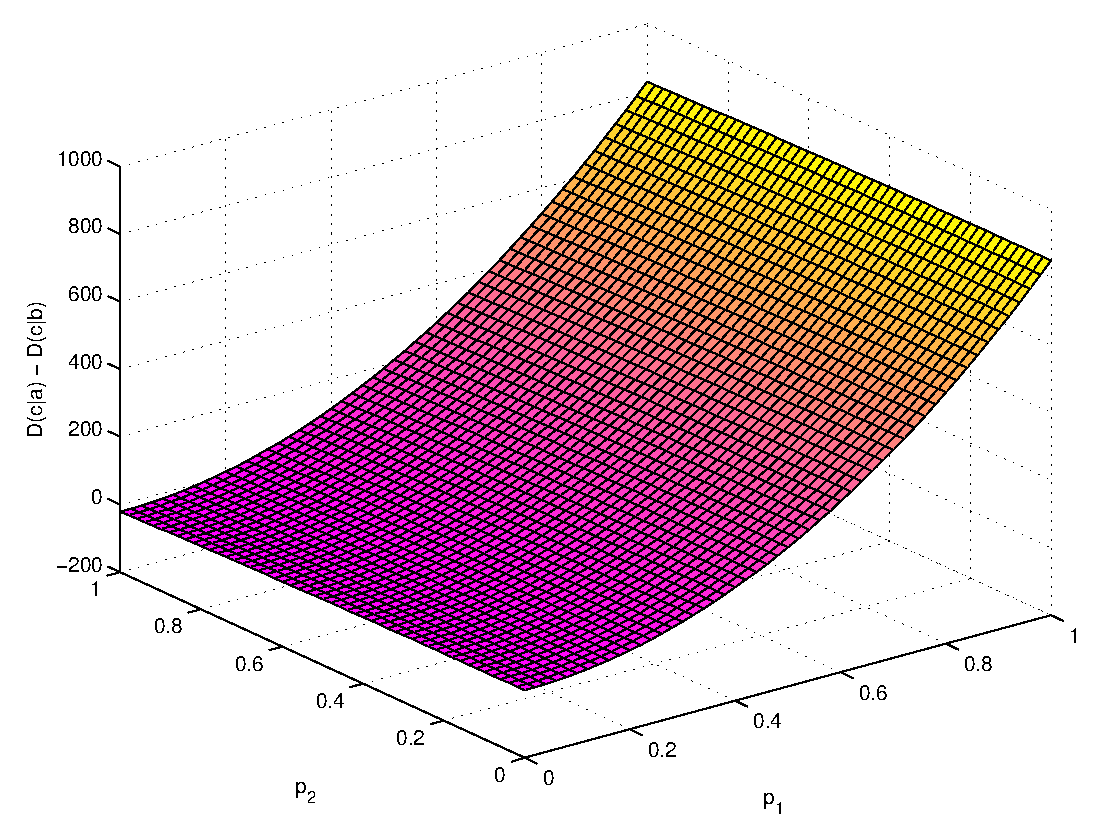
\includegraphics[width=1.0\textwidth]{variance_1.eps}
				\caption{Модель 1}
				\label{fig:variance_1}
				\end{subfigure}
				\begin{subfigure}[b]{0.5\textwidth}
					\centering
					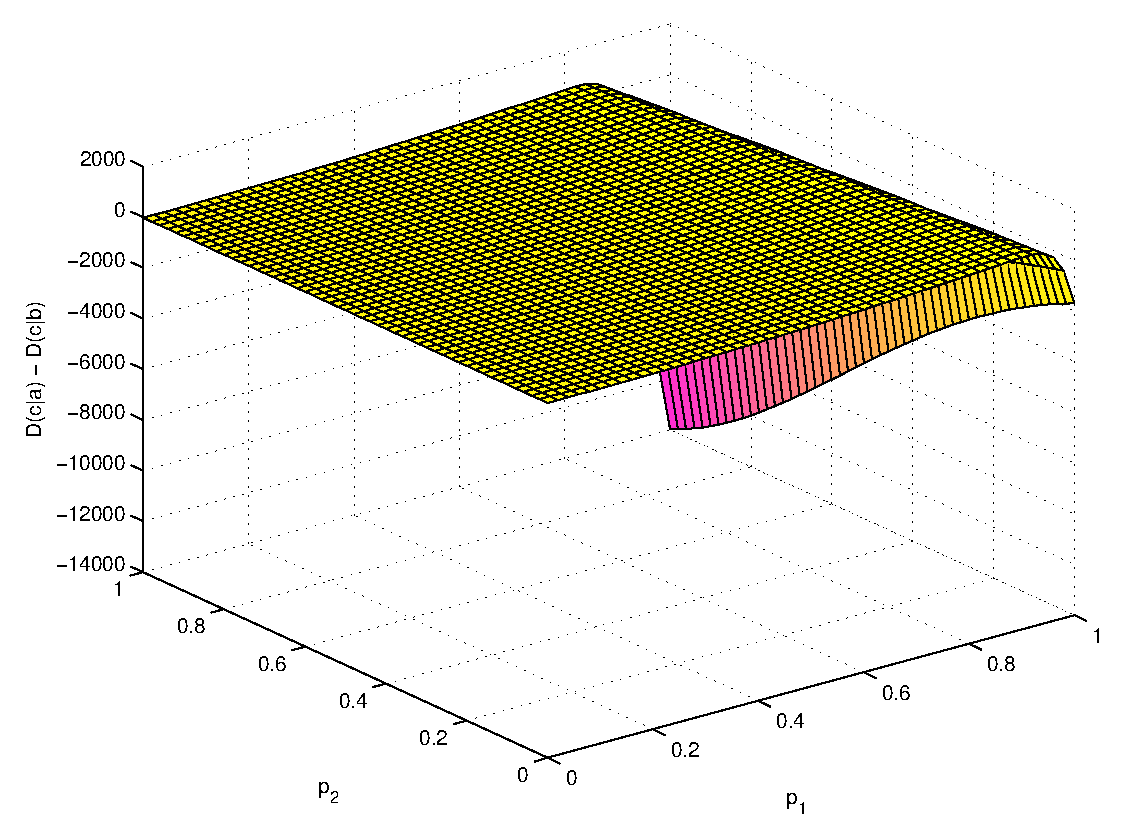
\includegraphics[width=1.0\textwidth]{variance_2.eps}
					\caption{Модель 2}
					\label{fig:variance_2}
				\end{subfigure}
				\captionsetup{justification=centering}
				\caption{Зависимость $\mathbb{D}[c|a] - \mathbb{D}[c|b]$ от $p_1$ и $p_2$ для моделей 1 и 2}
				\label{fig:distr_c_d}
			\end{figure}\par
			%Анализируя данное поведение дисперсий, можно сделать вывод, что изменение параметров $p_1$ и $p_2$ может привести к сильному расхождению моделей. Таким образом, приближённую модель стоит использовать лишь при ограниченном наборе параметров.\par
			Очевидно, что области $\{(p_1, p_2) | \mathbb{D}[c|a] \leqslant \mathbb{D}[c|b] \}$ и $\{(p_1, p_2) | \mathbb{D}[c|a] > \mathbb{D}[c|b] \}$ в модели 2 не являются линейно разделимыми. Результаты модели 1 не являются достаточно наглядными и требуют большего анализа.\par
			Найдём 3 точки на границе областей и проверим, лежат ли они на одной прямой. Для значений $p_1 = 0.05, 0.5$ и $0.95$ вычислим соответствующие $p_2$ с помощью бинарного поиска с критерием останова $|\mathbb{D}[c|a] - \mathbb{D}[c|b]| < 10^{-7}$. В таблице \ref{tab:3points} представлены координаты точек и значение разности дисперсий в них.
			\begin{table}[H]
				\centering
				\begin{tabular}{|c|c|c|c|}
					\hline
					Точка & $p_1$ & $p_2$ & $\mathbb{D}[c|a] - \mathbb{D}[c|b], 10^{-8}$\\
					\hline
					$z_1$ & 0.05 & 0.0095100594 & 4.46\\
					\hline
					$z_2$ & 0.5 & 0.0799816155 & 0.12\\
					\hline
					$z_3$ & 0.95 & 0.1503011680 & -7.21 \\
					\hline
				\end{tabular}
				\caption{Граничные точки}
				\label{tab:3points}
			\end{table}\par
			Cоставим 2 вектора, $v_1 = z_2 - z_1$ и $v_2 = z_3 - z_2$, и проверим их на коллинеарность. Получим $v_1 = (0.45, 0.07047), v_2 = (0.45, 0.07032).$ Поскольку координаты граничных точек вычислены с высокой степенью точности, то различие координат векторов в 4-м знаке даёт повод утверждать, что они неколлинеарны, следовательно, кривая, разделяющая области, не является прямой.
		\section{Временные замеры}
			Требуется рассчитать распределения $p(c), p(c|a), p(c|b), p(b|a), p(b|a,\,d), p(d)$. Значения параметров $a, b$ и $d$ положены равными их матожиданию ($a = 23, b = 300, d = 39$).\par
			Замеры производятся для полного набора выходных аргументов функций. Результаты представлены в таблице \ref{tab:time_results}.
			\begin{table}[H]
				\centering
				\begin{tabular}{|c|c|c|}
					\hline
					\multirow{2}{*}{Распределение} & \multicolumn{2}{|c|}{Время, с}\\
					\cline{2-3}
					& Модель 1 & Модель 2\\
					\hline
					$p(c)$ & 0.183 & 0.022\\
					\hline
					$p(c|a)$ & 0.107 & 0.013\\
					\hline
					$p(c|b)$ & 0.038 & 0.007\\
					\hline
					$p(b|a)$ & 0.001 & -\\
					\hline
					$p(b|a,\,d)$ & 0.106 & 0.028\\
					\hline
					$p(d)$ & 0.259 & 0.101\\
					\hline
				\end{tabular}
				\caption{Временные замеры}
				\label{tab:time_results}
			\end{table}\par
			\begin{figure}[H]
				\begin{subfigure}[b]{0.5\textwidth}
					\centering
					\includegraphics[width=1.0\textwidth]{p_c_a.eps}
					\caption{$p(c|a)$}
					\label{fig:distr_c_a}
				\end{subfigure}
				\begin{subfigure}[b]{0.5\textwidth}
					\centering
					\includegraphics[width=1.0\textwidth]{p_c_b.eps}
					\caption{$p(c|b)$}
					\label{fig:distr_c_b}
				\end{subfigure}
				\captionsetup{justification=centering}
				\caption{Распределения $p(c|a)$ и $p(c|b)$ для моделей 1 и 2}
				\label{fig:distr_c_cond}
			\end{figure}
	\section{Сравнение моделей 1 и 2}
		При больших значениях параметров $p_1$ и $p_2$ и малом числе испытаний (параметрах $a, b$) пуассоновское распределение недостаточно хорошо приближает сумму биномиальных. В этом можно убедиться, положив значения параметров $a_{min} = 1, a_{max} = 5, b_{min} = 10, b_{max} = 15, p_1 = 0.9$, см. рис. \ref{fig:distr_c_extr}:
			\begin{figure}[H]
				\captionsetup{justification=centering}
				\includegraphics[width=1.0\textwidth]{p_c_extr.jpg}
				\caption{Распределение $p(c)$ для моделей 1 и 2}
				\label{fig:distr_c_extr}
			\end{figure}\par
\end{document}